\chapter{Contribuciones}

En el cap\'itulo anterior presentamos c\'omo generar los tractogramas y el 
estado del arte para agruparlos. En este cap\'itulo presentamos las contribuciones
de nuestro trabajo. Comenzamos con una contribuci\'on menor que es estudiar la 
estabilidad del algoritmo de tractograf\'ia utilizado en el trabajo. Luego hacemos
un an\'alisis te\'orico del estado del arte y mostramos algunas de las 
problem\'aticas que posee. Finalmente utilizamos una funci\'on para transformar
los tractogramas al espacio eucl\'ideo y mostramos como esto permite mejorar tanto
la complejidad espacial como temporal del algoritmo de \textit{clustering}. \\

\section{Estudio de la convergencia de los tractogramas}
\label{sec:convergencia}

El diagrama de la figura \ref{fig:diagrama} divide el proceso de 
parcelaci\'on de la corteza en varios pasos. El tercero de ellos consiste
en generar tractogramas. Un tractograma para una semilla $s$ es una imagen
donde cada voxel $v$ representa la probabilidad de que $v$ est\'e 
conectado a $s$ mediante un conjunto de axones. En la secci\'on 
\ref{sec:tractogramas} presentamos una forma de crear tractogramas
mediante un procedimiento Monte Carlo generando \textit{streamlines}. Un
\textit{streamline} representa el movimiento aleatorio de una part\'icula
de agua dentro de la materia blanca. Los tractogramas creados de esta
manera son inherentemente estoc\'asticos. Esto genera algunas preguntas
interesantes: ¿Al repetir el experimento, podremos obtener el mismo
tractograma? y ¿Cu\'antas part\'iculas son necesarias para ello?. Para
contestar estas preguntas utilizamos la t\'ecnica estad\'istica de 
\textit{bootstrap} \cite{Efron1982}. \\

\settowidth\mylen{procedure2 tractograma(}
\addtolength\mylen{\parindent}

\begin{algorithm}[h!]
\caption{Algoritmo de tractograf\'ia utilizado}\label{alg:localtracking}
\begin{algorithmic}[1]

\Procedure{tractograma(anatomica: img. anat\'omica, \\ \hspace*{\mylen}
                              dMRI: img. de difusi\'on, \\ \hspace*{\mylen}
                              S: semilla, P: num. part\'iculas)}{}

\State \emph{csd} $\gets$ Constrained Spherical Deconvolution Model of \emph{dMRI}. 

\State \emph{mapa\_probabilistico} $\gets$ Mapa desde los coeficientes
                                           Spherical Harmonics en \emph{csd}

\State \emph{mapa\_visitas} $\gets$ matriz nula con mismas dimensiones que la anat\'omica

\For {p in [1$\dots$P]}

    \State $streamline_p$ $\gets \emptyset$
    \State \emph{posicion\_actual} $\gets$ posicion de S
    
    \While {posicion\_actual en materia blanca}

        \State \emph{direccion\_actual} $\gets$ elegir direccion desde
                                               \emph{mapa\_probabilistico} 
        
        \State \emph{posicion\_actual} $\gets$ avanzar solo un voxel en
                                               \emph{direccion\_actual} 
        
        \State $streamline_p$ $\gets$ agregar \emph{posicion\_actual}    
        
    \EndWhile
    
    \For {\emph{pos} in $streamline_p$}
        \State \emph{mapa\_visitas[pos]} $\gets$ \emph{mapa\_visitas[pos]} + 1
    \EndFor
    
\EndFor

\State \emph{tractograma} $\gets$
                                 \emph{log(mapa\_visitas+1)} / log(P+1)    

\State \Return \emph{tractograma} 
 
\EndProcedure

\end{algorithmic}
\label{alg:itract}
\end{algorithm}

\vspace{0.3cm}

\textit{Bootstrap} permite estimar la distribuci\'on de un estad\'istico
en base a calcularlo sobre remuestreos con repeticiones de una 
poblaci\'on. El m\'etodo es especialmente \'util cuando el n\'umero de
muestras que se posee no es significativamente alto. Nosotros queremos
estimar la distribuci\'on de la media de los \textit{tractogramas} en 
funci\'on de la cantidad de \textit{streamlines}. En la literatura
se usan hasta $100000$ \textit{streamlines} por cada semilla 
\cite{Anwander2006}. \textit{Bootstrap} nos permite realizar este estudio
con muchas menos. \\

Para entender mejor la relaci\'on entre \textit{streamlines} y
tractogramas presentamos en el algoritmo \ref{alg:itract} el pseudoc\'odigo
de la implementaci\'on de tractograf\'ia utilizada. Dicho algoritmo es una
instanciaci\'on del presentado en la secci\'on \ref{sec:tractogramas}. La
imagen de difusi\'on se enmarca en el modelo \textit{Constrained Spherical
Deconvolution} usando la forma propuesta por Aganj et al. 
\cite{Aganj2010}; el mapa de transiciones probabil\'isticas se recupera
usando \textit{Spherical Harmonics} \cite{Descoteaux2007} y el tractograma
se calcula usando la ecuaci\'on \ref{eq:normalizacion} propuesta en el 
trabajo de Moreno-Dominguez et al. \cite{Moreno-Dominguez2014}. \\

\begin{algorithm}
\caption{Procedimiento de \textit{Bootstraping}}\label{alg:localtracking}
\begin{algorithmic}[1]

\Procedure{estabilidad(S: semilla)}{}

\State \emph{streamlines} $\gets$ $\emptyset$

\Loop{ 15000 veces }
    \State \emph{stream} $\gets$ crear streamline desde S 
    \State \emph{streamlines} $\gets$ agregar \emph{stream}
\EndLoop

\State \emph{medias} $\gets$ $\emptyset$
\State \emph{varianzas} $\gets$ $\emptyset$

\For{\emph{ss\_size} in [200, 500, 800, $\dots$]}

    \State \emph{subsample} $\gets$ $\emptyset$

    \Loop{ 10000 veces }
        \State \emph{tractograma} $\gets$ tomar \emph{ss\_size} streams de
                                          \emph{streamlines} y crear
                                          tractograma
        \State \emph{subsample} $\gets$ agregar \emph{tractograma} 
    \EndLoop
    
    \State \emph{medias} $\gets$ agregar tractograma medio de 
                                 \emph{subsample}
    \State \emph{varianzas} $\gets$ agregar tractograma varianza de 
                                    \emph{subsample}
\EndFor

\State \Return \emph{medias}, \emph{varianzas} 
 
\EndProcedure

\end{algorithmic}
\label{alg:bootstrap}
\end{algorithm}

Usando el algoritmo \ref{alg:itract} generamos $15000$ 
\textit{streamlines} para distintas semillas en el \'area de Broca. Luego
calculamos el tractograma medio y la varianza de cada voxel utilizando
$10000$ submuestras aleatorias del mismo tama\~no. Repetimos esto con
varios tama\~nos de submuestra para estudiar la variabilidad del 
estad\'istico. Este procedimiento se puede ver en el algoritmo 
\ref{alg:bootstrap}.\\

Crear los tractogramas es uno de los pasos necesarios para parcelar la
corteza. Por la forma en que est\'an definidos, los tractogramas son
inherentemente estoc\'asticos. El m\'etodo aqu\'i presentado nos permite
estudiar la estabilidad del algoritmo de tractograf\'ia implementado. De
esta manera podemos comprobar si dado un n\'umero suficiente de 
part\'iculas los tractogramas de una semilla convergen a un mismo 
resultado. \\


\section{An\'alisis del m\'etodo Moreno-Dominguez}

Utilizar \textit{Hierarchical Agglomerative Clustering} con la distancia 
coseno y el \textit{linkage} centroide presenta al menos dos desventajas. 
Primero, la distancia coseno obliga a tener que comparar expl\'icitamente cada
centroide con los clusters existentes. Notemos que esto implica mantener los
clusters en memoria. Por otro lado, el promedio de probabilidades no
necesariamente representa una probabilidad \cite{Pohl2007}. Esto quiere decir
que el centroide de un grupo de tractogramas no necesariamente representa un
tractograma. \\

\subsection{Clustering de vectores colineales}

\begin{figure}[h!]
        \centering
        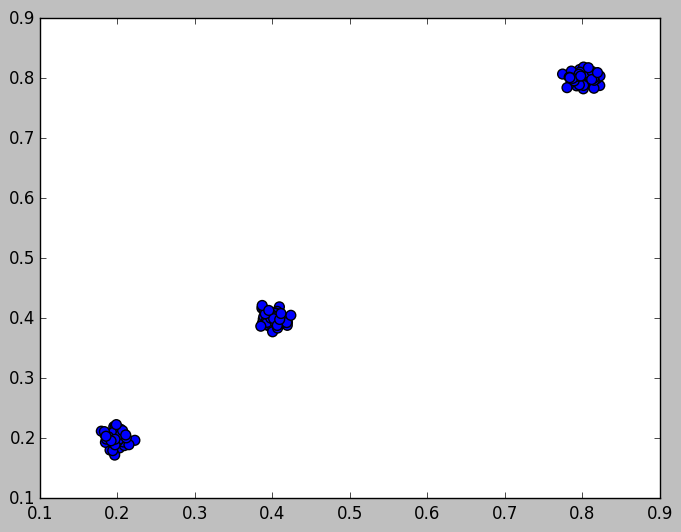
\includegraphics[width=0.5\textwidth]{img/3pop.png}
        \caption{Tres cluster colineales\-}
        \label{fig:3clusters}
\end{figure}

La distancia coseno es una forma de medir co\-rrelaci\'on entre vectores. Por ello,
cuando lo que se intenta agrupar son vectores colineales el resultado es aleatorio.
Por ejemplo, cuando se aplica el procedimiento sobre los puntos de la Figura
\ref{fig:3clusters} el resultado del clustering es la Figura \ref{fig:3moreno}.
Usando LogOdds y la m\'etrica euclidiana se consigue el \textit{clustering} de 
la Figura \ref{fig:3logit}.\\

\begin{figure}[h!]

\centering                                                                                                          
\begin{minipage}[b]{0.85\textwidth}
    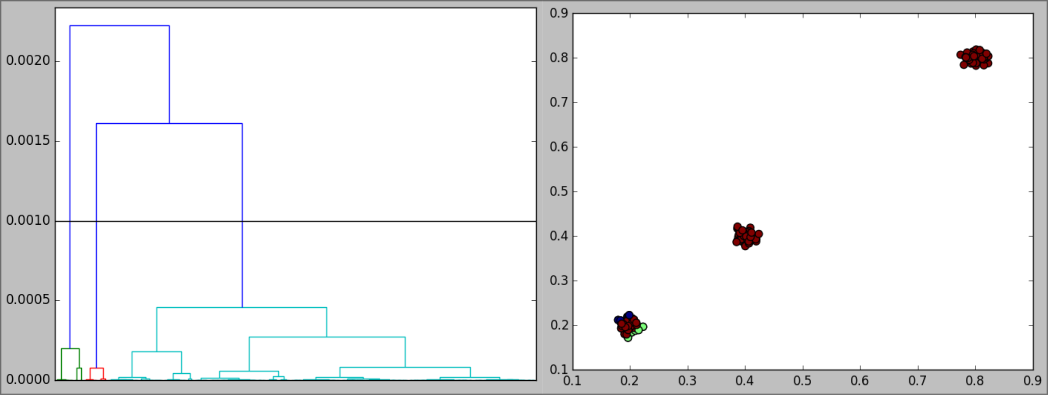
\includegraphics[width=\textwidth]{img/3pop_moreno.png}
    \caption{Clustering resultado de utilizar el m\'etodo Moreno}
    \label{fig:3moreno}
\end{minipage} ~

\end{figure}  

Los tractogramas son im\'agenes que por su naturaleza tienen muchos voxels con 
valores peque\~nos. La Figura \ref{fig:hist_tract} muestra el histograma de los
valores en los tractogramas del \'Area de Broca. Esta gran cantidad
de voxels con valores tan bajos podr\'ia generar ruido en las correlaciones.  

\begin{figure}[h!]
              \centering                                                                                                          
\begin{minipage}[b]{0.8\textwidth}
    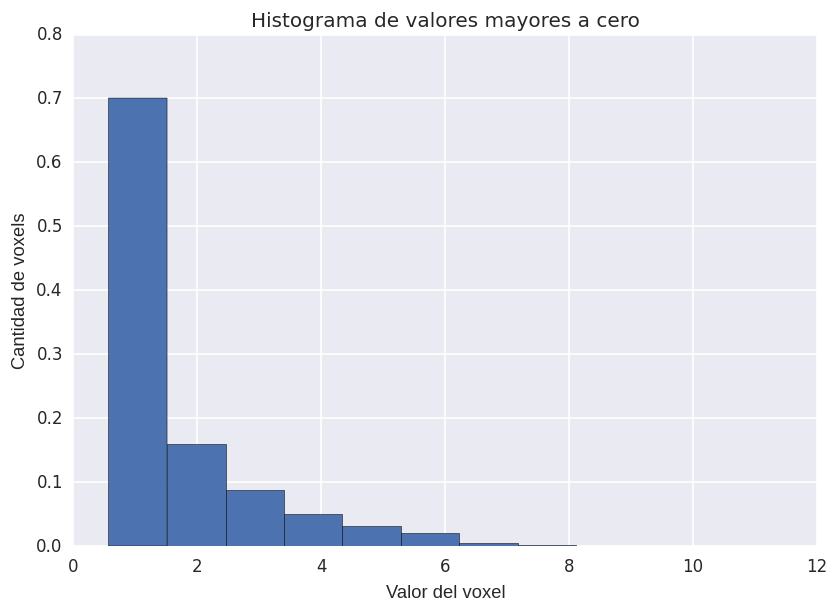
\includegraphics[width=\textwidth]{img/hist_tract.png}
    \caption{Histograma normalizado de los valores en los tractogramas del \'Area de Broca}
    \label{fig:hist_tract}
\end{minipage} ~

\end{figure}  


\subsection{Relaci\'on m\'etrica-\textit{linkage}}

La Figura \ref{fig:cos_cen} muestra cuatro vectores, sus posiciones en coordenadas
polares son: $ p_1 = (0.4, 45^\circ)$;  $p_2 = (0.3, 25^\circ)$;  $p_3 = (0.4, 66^\circ)$
y $p_4 = (0.4, 4.5^\circ) $ \\

Podemos apreciar que al principio $d(p_2,p_3) < d(p_3,p_4) < d(p_1,p_2)$, siendo
$d(x,y)$ la distancia coseno. Sin embargo, luego de utilizar el 
\textit{linkage centroid} sucede que $d(p_1,p_c) < d(p_4,p_c)$. $p_4$
es ahora el punto que mas lejos est\'a del centroide. Creando un representante
$p_m$ usando el \'angulo medio entre $p_2$ y $p_3$ esto no sucede. Este fen\'omeno
se da porque la distancia coseno tiene en cuenta el \'angulo pero el centroide
no. Por lo tanto el centroide no caracteriza al punto medio respecto a la
distancia coseno.\\

\begin{figure}[h!]
                                                                                                                        
\begin{minipage}[b]{\textwidth}
    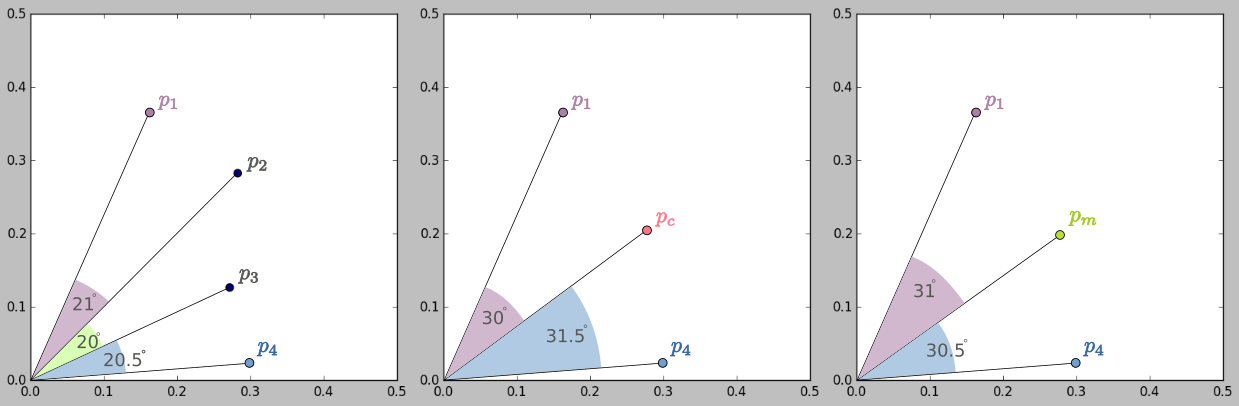
\includegraphics[width=\textwidth]{img/cosine_centroid.png}
    \caption{El centroide no representa el punto medio respecto al \'angulo}
    \label{fig:cos_cen}
\end{minipage} ~

\end{figure}  

\subsection{Complejidad algor\'itmica del clustering}

En todo el proceso el paso mas caro en t\'erminos computacionales es el
\textit{clustering}. En cada iteraci\'on del algoritmo es necesario comparar 
expl\'icitamente cada nuevo centroide con todo el resto de los clusters. Esto 
es costoso computacionalmente. Por cada iteraci\'on es necesario hacer $O(c^2 m)$
operaciones para recalcular todas las distancias, donde $c$ es la cantidad de
clusters y $m$ es la longitud de los mismos. Dadas $n$ semillas iniciales, la 
cantidad de iteraciones a realizar son $n-1$. La complejidad de este m\'etodo es
$O(n^3 m)$.



\section{Clustering en el Espacio Eucl\'ideo}

En la secci\'on anterior presentamos algunos de los inconvenientes te\'oricos 
del m\'etodo propuesto por Moreno-Dominguez. A continuaci\'on mostramos como 
solucionar todos ellos haciendo uso de la tranformaci\'on \textit{logit}. \\

\subsection{Transformaci\'on Logit}

Sea $P_M$ el espacio de una distribuci\'on discreta para $M$ etiquetas: 

$$P_M = \left\{  p | p = (p_1,\dots p_n) \in (0,1)^M , \sum{p_i} = 1 \right\}$$

La funci\'on \textit{logit}:$P_M \rightarrow R^{M-1}$ define una transformaci\'on
entre el espacio $P_M$ y el espacio eucl\'ideo $R^{M-1}$. Dados los vectores $Q \in P^M$ y
$S \in R^{M-1}$:

$$S_i = logit(Q_i) = log\left(\frac{Q_i}{Q_M}\right)$$

Para el caso de $M=2$ permite transformar la distribuci\'on Bernoulli
discreta al espacio eucl\'idio. Podemos ver en la ecuaci\'on \ref{eq:logit} su
expresi\'on anal\'itica y en la Figura \ref{fig:dominio} representaci\'on 
gr\'afica.

\begin{figure}[h!]

\begin{minipage}[b]{0.45\textwidth}

    \begin{equation}
    \vspace{2.85cm}
        \label{eq:logit}
    logit(p) = log\left(\frac{p}{1-p}\right)
    \end{equation}
\end{minipage} ~
\hfill
\begin{minipage}[b]{0.45\textwidth}
    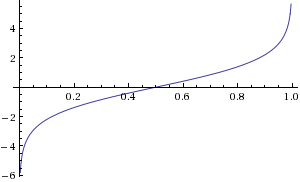
\includegraphics[width=\textwidth]{img/logit.png}
    \caption{Representaci\'on gr\'afica de la funci\'on logit}
    \label{fig:dominio}
\end{minipage} ~

\end{figure}  

Trabajar en el espacio eucl\'ideo nos asegura que la suma y la multiplicaci\'on
por escalares est\'an contenidos en el mismo espacio. Pohl et al. \cite{Pohl2007} 
utilizan esta propiedad para realizar operaciones lineales sobre mapas
probabil\'isticos. A su vez, demuestran que la suma y multiplicaci\'on
por escalares en el espacio eucl\'ideo poseen un significado en el espacio de la
distribuci\'on. \\

\subsection{Modificando el Algoritmo de Clustering}

Asumiendo que cada voxel $v$ de un tractograma proviene de la variable 
aleatoria binaria:

 $$X_v= \textrm{``La semilla est\'a conectada con el voxel v''}$$
 
Es posible transformar el tractograma aplicando la funci\'on \textit{logit} en
cada uno de sus voxels. El resultado es un vector donde cada coordenada se 
encuentra en el espacio eucl\'ideo.  M\'as a\'un, las operaciones lineales entre
los mismos voxels en distintos tractogramas est\'an definidas. Esto nos permite
usar la m\'etrica eucl\'ideana como funci\'on de similitud en \textit{Agglomerative
Hierarchical Clustering}. \\

Transformar de espacio los tractogramas y cambiar la funci\'on de similitud 
posee varias ventajas. Para empezar permite agrupar correctamente vectores
colineales. La Figura \ref{fig:3logit} muestra el resultado de aplicar este
m\'etodo a los vectores de la Figura \ref{fig:3clusters}.  Podemos apreciar 
que las tres poblaciones se encuentran correctamente separadas y bien definidas.\\

\begin{figure}[h!]

\centering
\begin{minipage}[b]{0.85\textwidth}
    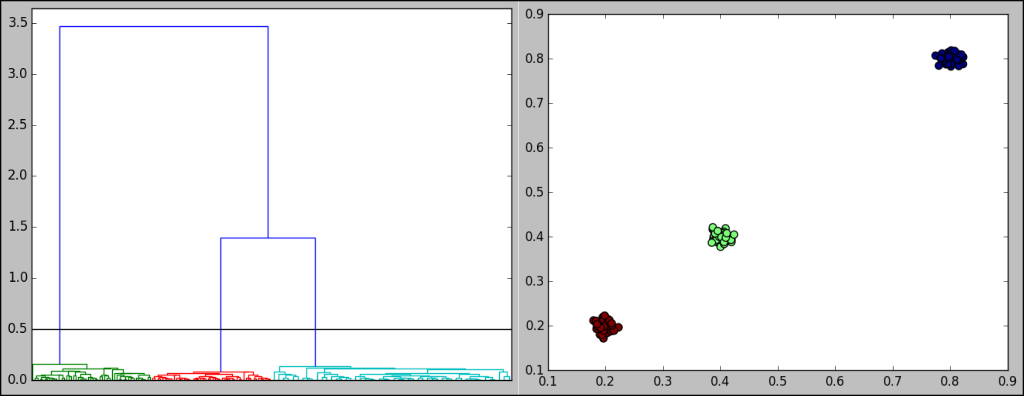
\includegraphics[width=\textwidth]{img/3pop_logit.png}
    \caption{Clustering resultado de utilizar el m\'etodo logit}
    \label{fig:3logit}
\end{minipage} ~

\end{figure}  

Otra ventaja es la buena relaci\'on m\'etrica-\textit{linkage}. Por definici\'on
el centroide es el centro de masa de los clusters. Esto quiere decir que es el 
punto que minimiza la distancia euclidiana entre los clusters que lo componen. 
Por ende, el centroide caracteriza bien el punto medio de los vectores en el
espacio eucl\'ideo. \\

Finalmente, nuestro m\'etodo tambi\'en permite mejorar la complejidad algor\'itmica.
Como ya explicamos, por cada iteraci\'on del algoritmo 
\textit{Agglomerative Herarchical Clustering} es necesario calcular un representante
de la uni\'on y luego computar su distancia al resto. Sin embargo, al usar la
m\'etrica euclideana junto con el \textit{linkage} centroide es posible simplificar
este paso. La formula de Lance y Williams permite computar las nuevas distancias
sin comparar expl\'icitamente los clusters. Esto baja significativamente la
complejidad. Cada iteraci\'on pasa a costar $O(c^2)$ en vez de $O(c^2 m)$, siendo
$c$ la cantidad de clusters y $m$ la longitud de los mismos. Dadas $n$ semillas 
iniciales, la complejidad temporal total del \textit{clustering} es $O(n^3)$. 
Con la distancia coseno era $O(n^3 m)$, siendo $m$ la longitud de los tractogramas.
Recordemos que en el contexto que estamos utilizando este algoritmo $m>>n$. Por
lo tanto, este resultado implica una gran mejora en la eficiencia del algoritmo.  


\subsection{Mejorando la Complejidad Espacial: Matrices Ralas}

Durante la etapa de \textit{clustering} es conveniente tener todos los
tractogramas en memoria. En nuestro caso, la matriz con los \textbf{tractogramas
sin transformar} del \'Area de Broca tiene dimensiones $762\times3587328$. 
Asumiendo que cada valor se representa usando $8$ Bytes, esta matriz ocupa un 
total de aproximadamente $20$ Gigabytes. Sin embargo, solo un $1\%$ de los datos
almacenados son no nulos. Esto implica que casi todo el espacio utilizado es
desperdiciado. \\

Es posible mejorar esto eliminando de la matriz las columnas que poseen solo
elementos nulos. La Figura \ref{fig:densa} muestra la matriz que resulta de
eliminar las columnas vacias de la matriz del \'Area de Broca. Si bien la nueva
matriz posee dimensiones $762\times121045$, a\'un solo el $27\%$ de los valores 
almacenados son no nulos. Manteniendo la representaci\'on de $8$ Bytes es posible
reducir el espacio necesario de $20$ Gigabites a aproximadamente $700$ Megabytes.\\

\begin{figure}[h!]
   \centering
    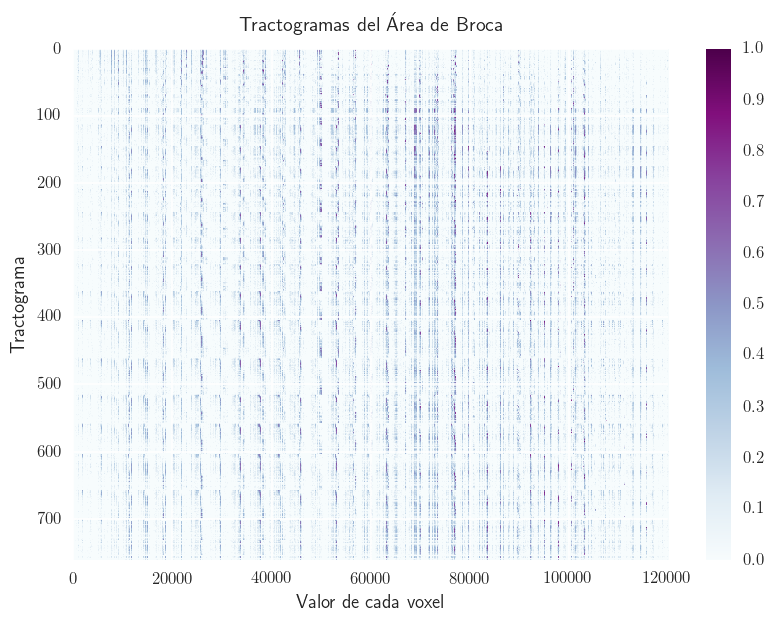
\includegraphics[width=0.9\textwidth]{img/densa_broca.png}
    \caption{Semillas en el hemisferio izquierdo. }
    \label{fig:densa}
\end{figure}

El problema de este \'ultimo m\'etodo es que a\'un desperdicia mucho espacio. En
el caso de utilizar todas los \textbf{tractogramas sin transformar} de un 
hemisferio, la matriz pasa a ser de dimensiones $21657\times3587328$ con un $1\%$
de valores no nulos. Para almacenar dicha matriz es necesario utilizar $587$ 
Gigabytes. Por esto es necesario utilizar estructuras mas eficiente, que aprovechen
lo ralo de las matrices. Ejemplos de estas estructuras son: \textit{Dictionary of
Keys}, o una matriz \textit{Compressed Sparse Row} (CSR). \\

%eliminando columnas in\'utiles nos queda 21657x145574, son 23.5 Gn

Si recordamos la forma que tiene la funci\'on logit encontramos un inconveniente
al querer utilizar matrices ralas. Podemos ver en la Figura \ref{fig:dominio} que
\textit{logit}$(0) = -\infty$. Esto implica que la transformaci\'on de una matriz
rala no es rala en t\'erminos de elementos nulos. Sin embargo podemos aprovechar
ciertas propiedades para recuperar las matrices ralas. La distancia euclidena 
entre vectores es invariante a traslaciones lineales del sistema. Lo mismo sucede
con las posiciones relativas de los centroides. Asignemos una representaci\'on 
finita $c$ al valor $-\infty$. Un buen candidato para $c$ es el $log(\epsilon)$,
donde $\epsilon$ es el \textit{epsilon de la maquina}. Transformar todos los vectores
y luego trasladarlos sumando $c$ en cada componente dara como resultado una
representaci\'on rala. Gracias a esto podemos utilizar DOK, CSR o cualquier
estructura para reducir los costos espaciales del clustering. \\








\blankpage
